%!TEX root = ..\MainFile.tex
\section{Результаты выполнения работы} % (fold)
\label{sec:WorkResults}	

В результате выполнения работы, нами были получены профили скорости (т.е. зависимость параметра порядка от высоты) для течения Куэтта идеальной самодвижущейся жидкости по модели Vicsek'a.

\begin{figure}
    \centering
        \begin{subfigure}
            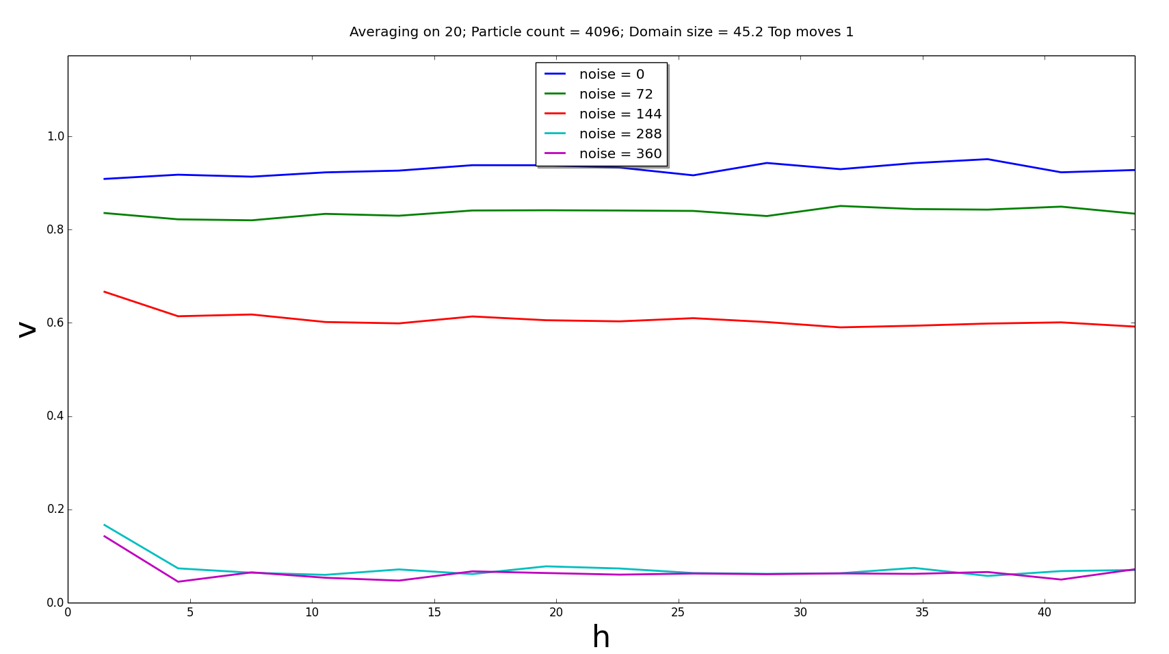
\includegraphics[height=\textheight/3]{Images/4k_x20}
            \caption{Число частиц: 4096; Плотность: 2; Число конфигураций: 20; Зеркальная граница}
            \label{fig:Results:32k}
        \end{subfigure}
        \begin{subfigure}{}
            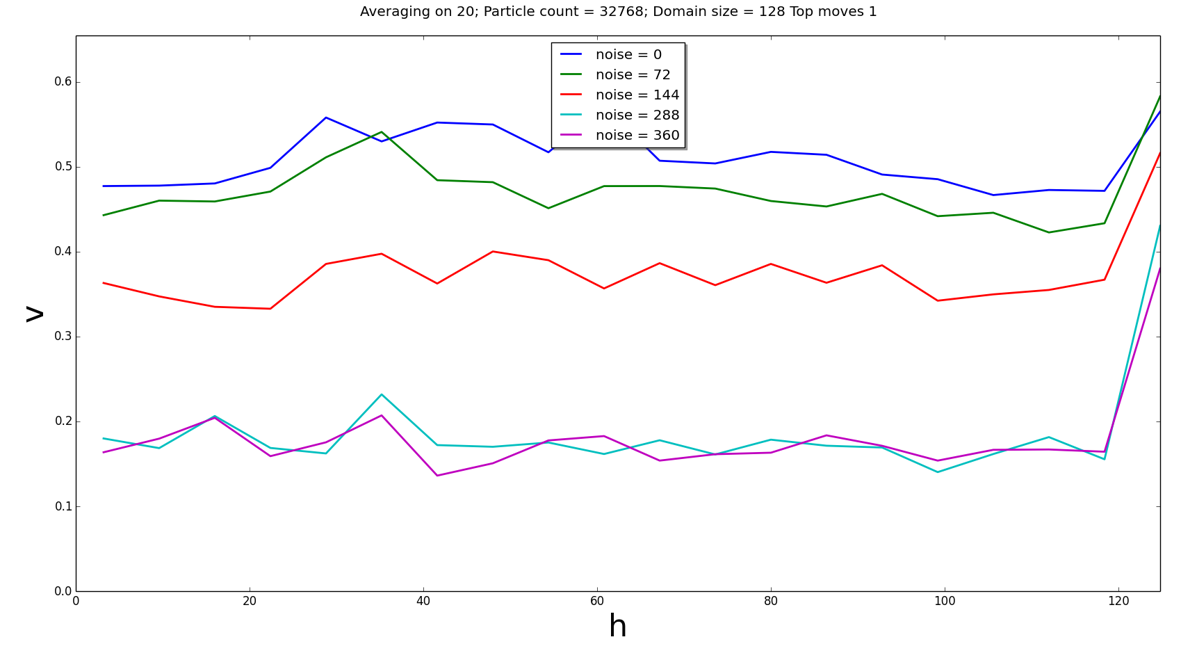
\includegraphics[height=\textheight/3]{Images/32k_x20}
            \caption{Число частиц: 32768; Плотность: 2; Число конфигураций: 20; Зеркальная граница}
            \label{fig:Results:32kOld}
        \end{subfigure}
        \begin{subfigure}{}
            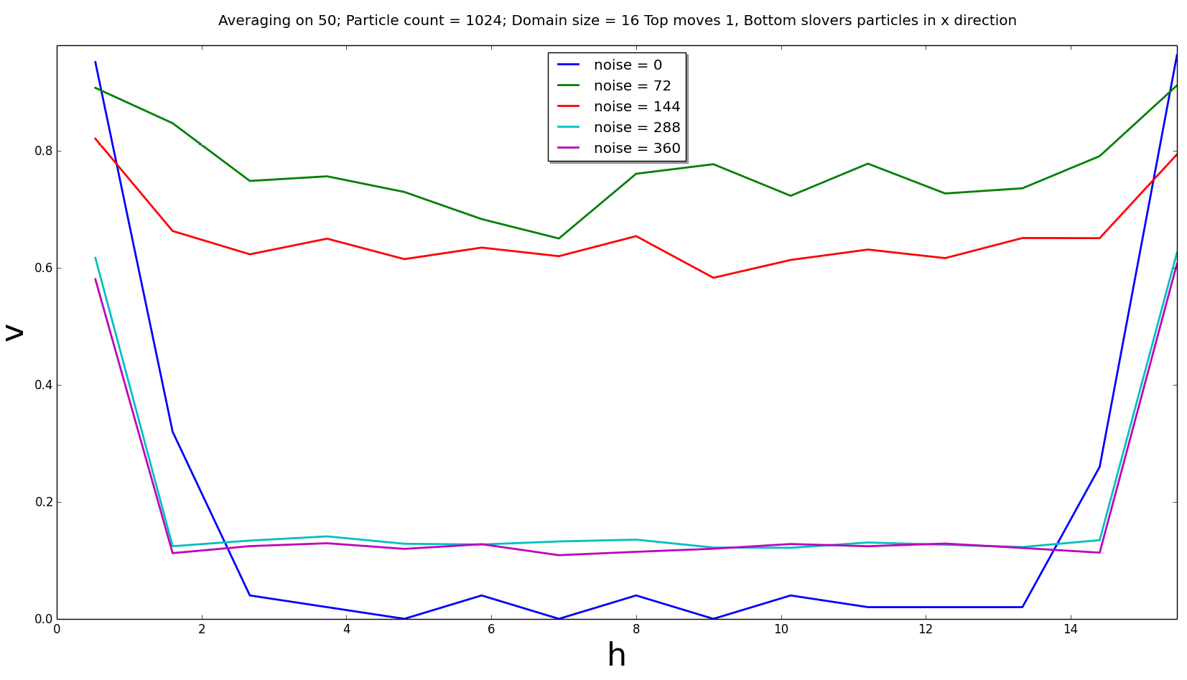
\includegraphics[height=\textheight/3]{Images/1k_x50_NotMirror}
            \caption{Число частиц: 1024; Плотность: 4; Число конфигураций: 50; Шероховатая граница}
            \label{fig:Results:4kNew}
        \end{subfigure}
    \caption{Зависимость параметра порядка от высоты для течения Куэтта при разных значениях шума.}
    \label{fig:Results}
\end{figure}

Предложенный алгоритм определения стабилизации состояния системы оправдал себя. Поскольку определение времени стабилизации не входило в тему данной работы, то специальных замеров не проводилось, но среднее значение времени симуляции для каждого значения шума составило $10^{2-3}$ по порядку величины, увеличиваясь с увеличением количества частиц.

Кроме того, были проведены более длительные симуляции для отдельных значений шума (в частности, очень большого и очень низкого). Полученные результаты не вошли в эту работу по причине того, что они аналогичны представленным на рис.~\ref{fig:Results}.

Побочным результатом выполнения работы также стало создание программы, способной выполнять симуляции идеальной самодвижущейся жидкости по модели Vicsek'a на GPU, и легко доступной для модернизации.
   
% section WorkResults (end)	